\documentclass[11pt, a4paper, reqno]{scrartcl}

\usepackage[utf8]{inputenc}
\usepackage{a4wide}
\usepackage{libertine}
\usepackage{graphicx}
\usepackage{listings}
\usepackage{xcolor}
\usepackage{float}
\usepackage{amsmath}

% for latex output of pandas
\usepackage{booktabs}

\begin{document}
    \title{Exercise No. 1}
    \author{David Bubeck, Pascal Becht, Patrick Nisbl\`e}
    \maketitle
    
    \lstset{
        language=Python,
        backgroundcolor=\color{gray!10},
        numbers=left,
        captionpos=t,
        breaklines=true,
        frame=l,
        xleftmargin=\parindent,
        basicstyle=\footnotesize\sffamily,
        keywordstyle=\bfseries\color{green!40!black},
        commentstyle=\itshape\color{purple!40!black},
        identifierstyle=\color{blue!60!black},
        stringstyle=\color{orange}
    }

    \newpage
    \section*{2 - Numerical Integration}
    
    We are to use 
    \begin{align}
        y_n(a)
            =\int_{0}^{1}\left(\frac{x^n}{x-a}\right)d\text x
            =\frac 1 n -a\cdot y_{n-1}(a)
    \end{align}
    for the following tasks
    \subsection*{a)}
    Plotting the Integrand for $n \in \{1,5,10,20,30,50\}$ and $x\in [0,1]$
    \begin{figure}[H]
        \lstinputlisting[language=Python,
        caption={
            01-2a.py
        },
        lastline=17]{01-2a.py}        
    \end{figure}
    
    \begin{figure}[H]
        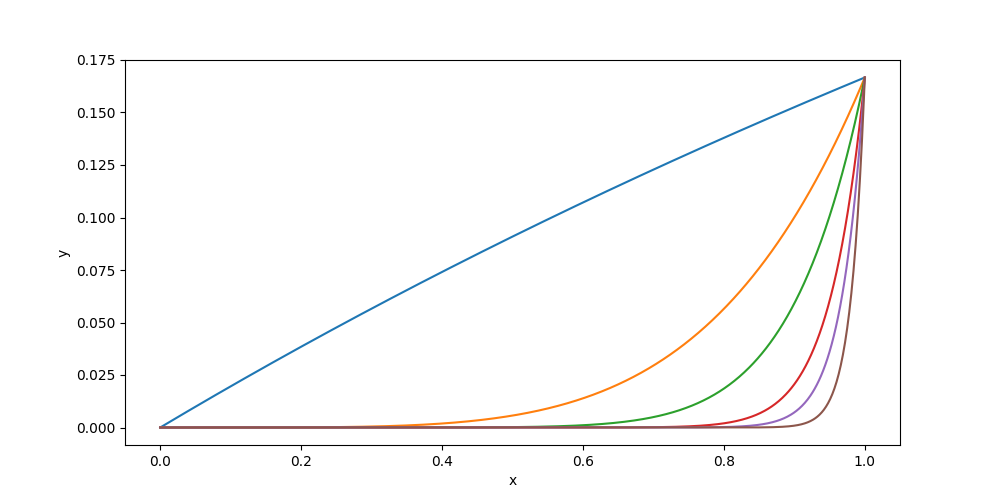
\includegraphics[width=.7\paperwidth]{01-2a}
        \caption{plotted integrand for given n and x interval}
    \end{figure}

    \newpage
    \subsection*{b)}
    Now for the Integration steps: iterate over a list between $n_0$ and $n_1$ starting at the lower, using a given $a$ and $y_0$  
    \lstinputlisting[
        lastline=50,
        caption={
            01-2b.py
        }]{01-2b.py}
    \begin{figure}[H]
        \centering
        \begin{tabular}{lrr}
\toprule
{} &     n &    $y_n(5.0)$ \\
\midrule
0  &   0.0 &  1.000000e+01 \\
1  &  10.0 & -4.990909e+01 \\
2  &  11.0 &  2.496288e+02 \\
3  &  12.0 & -1.248067e+03 \\
4  &  13.0 &  6.240407e+03 \\
5  &  14.0 & -3.120197e+04 \\
6  &  15.0 &  1.560099e+05 \\
7  &  16.0 & -7.800494e+05 \\
8  &  17.0 &  3.900247e+06 \\
9  &  18.0 & -1.950124e+07 \\
10 &  19.0 &  9.750618e+07 \\
11 &  20.0 & -4.875309e+08 \\
12 &  21.0 &  2.437654e+09 \\
13 &  22.0 & -1.218827e+10 \\
14 &  23.0 &  6.094136e+10 \\
15 &  24.0 & -3.047068e+11 \\
16 &  25.0 &  1.523534e+12 \\
17 &  26.0 & -7.617670e+12 \\
18 &  27.0 &  3.808835e+13 \\
19 &  28.0 & -1.904418e+14 \\
20 &  29.0 &  9.522088e+14 \\
21 &  30.0 & -4.761044e+15 \\
\bottomrule
\end{tabular}
    
        \caption{output of 01-2b.py}
    \end{figure}

    \newpage
    \subsection*{c)}
    repeat b) with given values
    
    \lstinputlisting[
        caption={
            01-2c.py
        }
    ]{01-2c.py}
    
    \begin{figure}[H]
        \centering
        \begin{tabular}{lrr}
\toprule
{} &     n &       $y_n(5)$ \\
\midrule
0  &   0.0 &       0.182322 \\
1  &   0.0 &       0.088392 \\
2  &   1.0 &       0.058039 \\
3  &   2.0 &       0.043139 \\
4  &   3.0 &       0.034306 \\
5  &   4.0 &       0.028468 \\
6  &   5.0 &       0.024325 \\
7  &   6.0 &       0.021233 \\
8  &   7.0 &       0.018837 \\
9  &   8.0 &       0.016926 \\
10 &   9.0 &       0.015368 \\
11 &  10.0 &       0.014071 \\
12 &  11.0 &       0.012977 \\
13 &  12.0 &       0.012040 \\
14 &  13.0 &       0.011229 \\
15 &  14.0 &       0.010522 \\
16 &  15.0 &       0.009890 \\
17 &  16.0 &       0.009372 \\
18 &  17.0 &       0.008696 \\
19 &  18.0 &       0.009151 \\
20 &  19.0 &       0.004243 \\
21 &  20.0 &       0.026406 \\
22 &  21.0 &      -0.086575 \\
23 &  22.0 &       0.476352 \\
24 &  23.0 &      -2.340094 \\
25 &  24.0 &      11.740469 \\
26 &  25.0 &     -58.663883 \\
27 &  26.0 &     293.356454 \\
28 &  27.0 &   -1466.746558 \\
29 &  28.0 &    7333.767272 \\
30 &  29.0 &  -36668.803026 \\
31 &  30.0 &  183344.047389 \\
\bottomrule
\end{tabular}

        \caption{output of 01-2c.py}
    \end{figure}

    \begin{figure}[H]
        \centering
        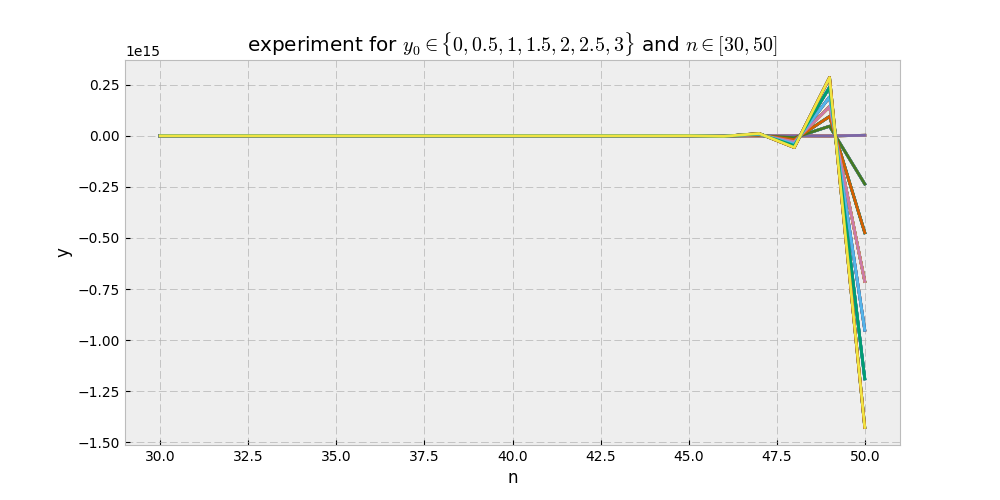
\includegraphics[width=.8\paperwidth]{01-2c}
    \end{figure}
    
    
    
\end{document}